\documentclass[border={0pt 0pt 0pt 0pt}]{standalone}

\usepackage{hyperref}
\usepackage{tikz}

\usetikzlibrary{decorations.pathreplacing,
  arrows,
  calc,
  decorations.pathmorphing,
  decorations.pathreplacing,
  decorations.markings,
  positioning,
  shapes,
  3d
}
\usepgfmodule{oo}

\ifpdf
% Ensure reproducible output
\pdfinfoomitdate=1
\pdfsuppressptexinfo=-1
\pdftrailerid{}
\hypersetup{
  pdfcreator={},
  pdfproducer={}
}
\fi

\pgfdeclarelayer{tweezer}
\pgfsetlayers{tweezer,main}
\pgfooclass{tweezer}{
  \method tweezer() {
  }
  \method drawNaAtom(#1,#2,#3) {
    \pgfgettransformentries{\myscaleX}{\mytmp}{\mytmp}{\myscaleY}{\mytmp}{\mytmp}
    \node at (#1, #2) {\scalebox{\myscaleX}[\myscaleY]{\scalebox{#3}{
          
\includegraphics[width=2cm]{fadings/na_atom.png}}}};
  }
  \method drawCsAtom(#1,#2,#3) {
    \pgfgettransformentries{\myscaleX}{\mytmp}{\mytmp}{\myscaleY}{\mytmp}{\mytmp}
    \node at (#1, #2) {\scalebox{\myscaleX}[\myscaleY]{\scalebox{#3}{
          
\includegraphics[width=2cm]{fadings/cs_atom.png}}}};
  }
  \method drawNaTweezer(#1,#2) {
    \begin{pgfonlayer}{tweezer}
      \begin{scope}[shift={(#1,#2)}]
        \pgfgettransformentries{\myscaleX}{\mytmp}{\mytmp}{\myscaleY}{\mytmp}{\mytmp}
        \clip[rotate=90] plot[draw,samples=200,domain=-1.5:1.5] function {sqrt(0.01 + x**2 / 5)}
        -- plot[draw,samples=200,domain=1.5:-1.5] function {-sqrt(0.01 + x**2 / 5)};
        \node[rotate=90] at (0, 0)
        {\scalebox{\myscaleX}[\myscaleY]{
            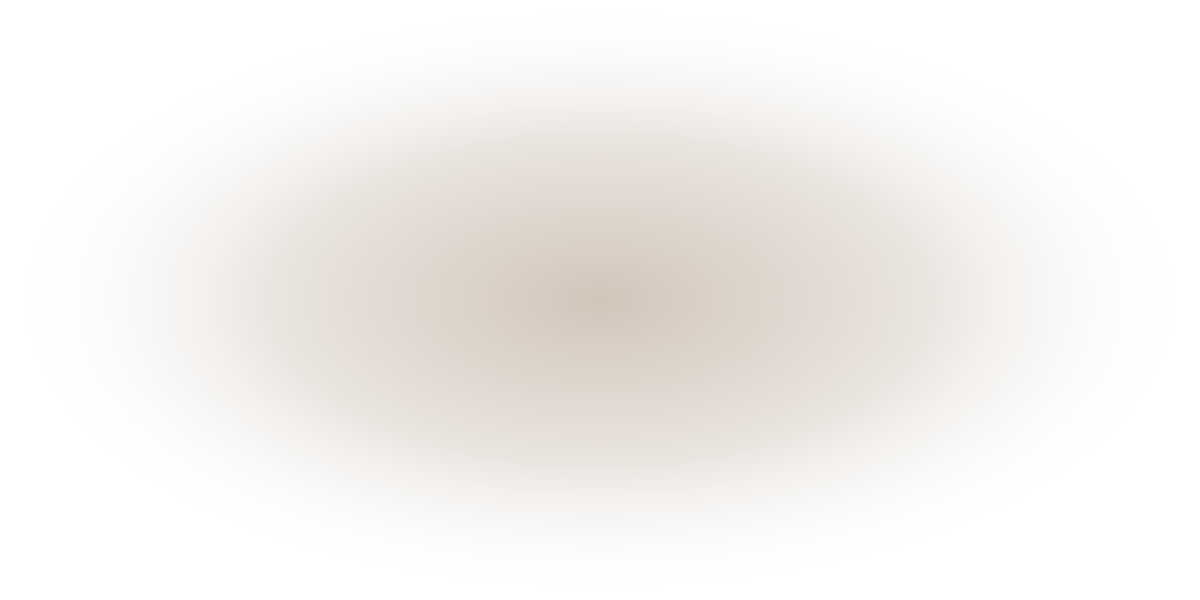
\includegraphics[height=1.356466cm,width=3cm]{fadings/na_tweezer.png}}};
      \end{scope}
    \end{pgfonlayer}
  }
  \method drawCsTweezer(#1,#2) {
    \begin{pgfonlayer}{tweezer}
      \begin{scope}[shift={(#1,#2)}]
        \pgfgettransformentries{\myscaleX}{\mytmp}{\mytmp}{\myscaleY}{\mytmp}{\mytmp}
        \clip[rotate=90] plot[draw,samples=200,domain=-1.5:1.5] function {sqrt(0.01 + x**2 / 5)}
        -- plot[draw,samples=200,domain=1.5:-1.5] function {-sqrt(0.01 + x**2 / 5)};
        \node[rotate=90] at (0, 0)
        {\scalebox{\myscaleX}[\myscaleY]{
            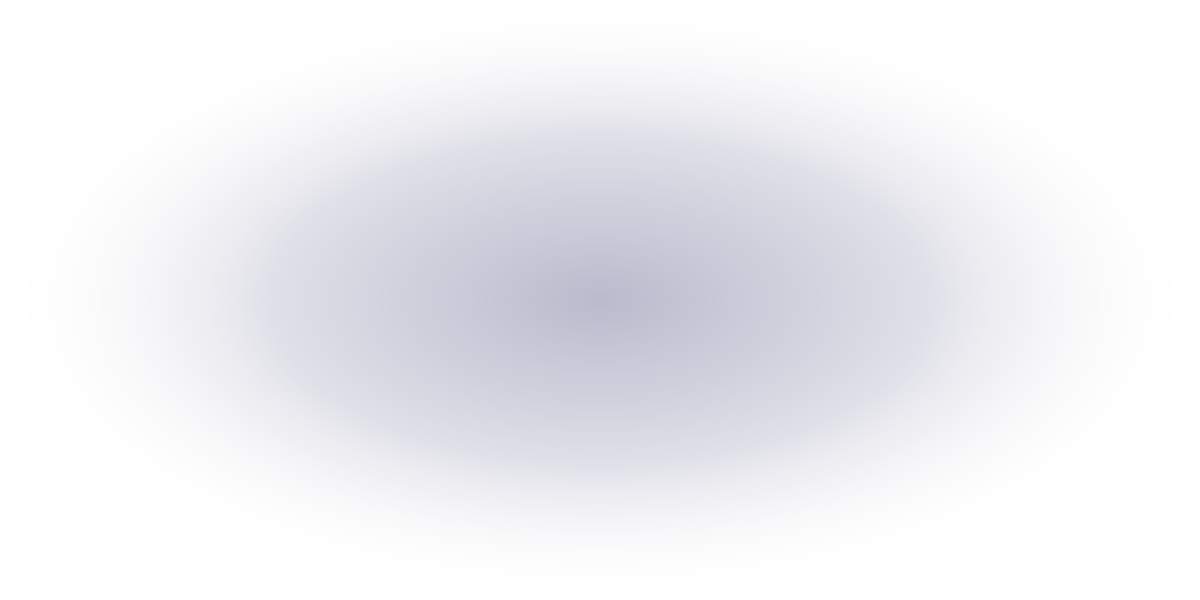
\includegraphics[height=1.356466cm,width=3cm]{fadings/cs_tweezer.png}}};
      \end{scope}
    \end{pgfonlayer}
  }
}
\pgfoonew \mytweezer=new tweezer()

\begin{document}
\begin{tikzpicture}[scale=1.2]
  \node[left,align=center] at (-1.5, 2.4) {\textbf{Loading and}\\\textbf{Cooling}};
  \node[left] at (-1.5, 0) {\textbf{Merging}};
  \node[left,align=center] at (-1.5, -2.4) {\textbf{Weakly Bound}\\\textbf{Molecules}};
  \node[left,align=center] at (-1.5, -4.8) {\textbf{Rovibronic Ground}\\\textbf{State Molecules}};
  \foreach \x in {0, 1, 2} {
    \begin{scope}[shift={(\x * 3.0, 0)}]
      \draw[->,>=stealth,orange,dotted,line width=1.2,opacity=0.7] (-1, 2.2) -- (-1, 0.2);
      \draw[->,>=stealth,blue,dotted,domain=1.0:-1.0,
      smooth,variable=\y,line width=1.2,opacity=0.7]
      plot ({atan(\y * 6.5) / 170 - 0.5},{\y + 1.2});

      \foreach \y in {1, 2} {
        \begin{scope}[shift={(0, -2.4 * \y)}]
          \draw[->,>=stealth,blue!50!orange,dotted,line width=1.2] (-1, 2.2) -- (-1, 0.2);
        \end{scope}
      }

      \begin{scope}[shift={(0, 2.4)}]
        \mytweezer.drawCsTweezer(0, 0)
        \mytweezer.drawNaTweezer(-1, 0)
        \mytweezer.drawCsAtom(0.0, 0, 0.089)
        \mytweezer.drawNaAtom(-1.0, 0, 0.11)
      \end{scope}

      \begin{scope}[shift={(0, 0)}]
        \mytweezer.drawCsTweezer(-1, 0)
        \mytweezer.drawNaAtom(-1.10, 0.05, 0.11)
        \mytweezer.drawCsAtom(-0.90, -0.05, 0.089)
      \end{scope}

      \begin{scope}[shift={(0, -2.4)}]
        \mytweezer.drawCsTweezer(-1, 0)
        \draw[line width=1] (-1.07, 0.075) -- (-0.93, -0.075);
        \mytweezer.drawNaAtom(-1.07, 0.075, 0.11)
        \mytweezer.drawCsAtom(-0.93, -0.075, 0.089)
      \end{scope}

      \begin{scope}[shift={(0, -4.8)}]
        \mytweezer.drawCsTweezer(-1, 0)
        \draw[line width=1] (-1 - 0.07 * 0.7, 0.075 * 0.7) -- (-1 + 0.07 * 0.7, -0.075 * 0.7);
        \mytweezer.drawNaAtom(-1 - 0.07 * 0.7, 0.075 * 0.7, 0.11)
        \mytweezer.drawCsAtom(-1 + 0.07 * 0.7, -0.075 * 0.7, 0.089)
      \end{scope}
    \end{scope}
  }
\end{tikzpicture}
\end{document}
